%===============================================================================
% LaTeX sjabloon voor de bachelorproef toegepaste informatica aan HOGENT
% Meer info op https://github.com/HoGentTIN/latex-hogent-report
%===============================================================================

\documentclass[dutch,dit,thesis]{hogentreport}

% TODO:
% - If necessary, replace the option `dit`' with your own department!
%   Valid entries are dbo, dbt, dgz, dit, dlo, dog, dsa, soa
% - If you write your thesis in English (remark: only possible after getting
%   explicit approval!), remove the option "dutch," or replace with "english".

\usepackage{lipsum} % For blind text, can be removed after adding actual content

%% Pictures to include in the text can be put in the graphics/ folder
\graphicspath{{graphics/}}

%% For source code highlighting, requires pygments to be installed
%% Compile with the -shell-escape flag!
\usepackage[section]{minted}
%% If you compile with the make_thesis.{bat,sh} script, use the following
%% import instead:
%% \usepackage[section,outputdir=../output]{minted}
\usemintedstyle{solarized-light}
\definecolor{bg}{RGB}{253,246,227} %% Set the background color of the codeframe

%% Change this line to edit the line numbering style:
\renewcommand{\theFancyVerbLine}{\ttfamily\scriptsize\arabic{FancyVerbLine}}

%% Macro definition to load external java source files with \javacode{filename}:
\newmintedfile[javacode]{java}{
    bgcolor=bg,
    fontfamily=tt,
    linenos=true,
    numberblanklines=true,
    numbersep=5pt,
    gobble=0,
    framesep=2mm,
    funcnamehighlighting=true,
    tabsize=4,
    obeytabs=false,
    breaklines=true,
    mathescape=false
    samepage=false,
    showspaces=false,
    showtabs =false,
    texcl=false,
}

% Other packages not already included can be imported here

%%---------- Document metadata -------------------------------------------------
% TODO: Replace this with your own information
\author{Alif Monnoye}
\supervisor{Dhr. L. Blondeel}
\cosupervisor{Dhr. N. Sletten}
\title[]%
    {PoC: Opzetten van Pydev in IBM Developer for z/OS om Python programma's uit te voeren op de mainframe}
\academicyear{\advance\year by -1 \the\year--\advance\year by 1 \the\year}
\examperiod{1}
\degreesought{\IfLanguageName{dutch}{Professionele bachelor in de toegepaste informatica}{Bachelor of applied computer science}}
\partialthesis{false} %% To display 'in partial fulfilment'
\institution{Den Norske Bank (DNB)}

%% Add global exceptions to the hyphenation here
\hyphenation{back-slash}

%% The bibliography (style and settings are  found in hogentthesis.cls)
\addbibresource{bachproef.bib}            %% Bibliography file
\addbibresource{../voorstel/voorstel.bib} %% Bibliography research proposal
\defbibheading{bibempty}{}

%% Prevent empty pages for right-handed chapter starts in twoside mode
\renewcommand{\cleardoublepage}{\clearpage}

\renewcommand{\arraystretch}{1.2}

%% Content starts here.
\begin{document}

%---------- Front matter -------------------------------------------------------

\frontmatter

\hypersetup{pageanchor=false} %% Disable page numbering references
%% Render a Dutch outer title page if the main language is English
\IfLanguageName{english}{%
    %% If necessary, information can be changed here
    \degreesought{Professionele Bachelor toegepaste informatica}%
    \begin{otherlanguage}{dutch}%
       \maketitle%
    \end{otherlanguage}%
}{}

%% Generates title page content
\maketitle
\hypersetup{pageanchor=true}

%%=============================================================================
%% Voorwoord
%%=============================================================================

\chapter*{\IfLanguageName{dutch}{Woord vooraf}{Preface}}%
\label{ch:voorwoord}

%% TODO:
%% Het voorwoord is het enige deel van de bachelorproef waar je vanuit je
%% eigen standpunt (``ik-vorm'') mag schrijven. Je kan hier bv. motiveren
%% waarom jij het onderwerp wil bespreken.
%% Vergeet ook niet te bedanken wie je geholpen/gesteund/... heeft

Dit is een proof of concept die ik wil uitwerken omdat dit hulp kan bieden in de modernisatie van de mainframe systemen van IBM. Op het moment van schrijven heb ik al stage gedaan bij 2 bedrijven die gebruik maken van een mainframe en deze gebruiken allebei IBM Developer for zOS om applicaties te schrijven in verschillende soorten programmeertalen zoals COBOL, PL/1, Python, Java, ... Python is één van de meest gebruikte programmeertalen op de dag van vandaag en hierin wordt dus veel ingezet door IBM om deze programmeertaal zo efficiënt mogelijk te laten werken op hun systemen. De skills in de `oudere` programmeertalen zoals COBOL en PL/1 is sterk aan het afnemen dus is de inbreng van Python bijna een must om nog goede programmeurs te vinden. Een goede editor is ook nodig wat momenteel niet het geval is in IDz dus maak ik in dit onderzoek een stappenplan om dit zo goed mogelijk op te stellen.
\\ \\
Ik zou Njaal Sletten en Stian Botnevik van DNB, Noorwegen willen bedanken voor de hulp en inspiratie bij het schrijven en uitwerken van dit onderzoek. Ze hielpen allebei met het technische gedeelte en Stian kwam met de probleemstelling.
%%=============================================================================
%% Samenvatting
%%=============================================================================

% TODO: De "abstract" of samenvatting is een kernachtige (~ 1 blz. voor een
% thesis) synthese van het document.
%
% Een goede abstract biedt een kernachtig antwoord op volgende vragen:
%
% 1. Waarover gaat de bachelorproef?
% 2. Waarom heb je er over geschreven?
% 3. Hoe heb je het onderzoek uitgevoerd?
% 4. Wat waren de resultaten? Wat blijkt uit je onderzoek?
% 5. Wat betekenen je resultaten? Wat is de relevantie voor het werkveld?
%
% Daarom bestaat een abstract uit volgende componenten:
%
% - inleiding + kaderen thema
% - probleemstelling
% - (centrale) onderzoeksvraag
% - onderzoeksdoelstelling
% - methodologie
% - resultaten (beperk tot de belangrijkste, relevant voor de onderzoeksvraag)
% - conclusies, aanbevelingen, beperkingen
%
% LET OP! Een samenvatting is GEEN voorwoord!

%%---------- Nederlandse samenvatting -----------------------------------------
%
% TODO: Als je je bachelorproef in het Engels schrijft, moet je eerst een
% Nederlandse samenvatting invoegen. Haal daarvoor onderstaande code uit
% commentaar.
% Wie zijn bachelorproef in het Nederlands schrijft, kan dit negeren, de inhoud
% wordt niet in het document ingevoegd.

%\IfLanguageName{english}{%
%\selectlanguage{dutch}
%\chapter*{Samenvatting}
%\lipsum[1-4]
%\selectlanguage{english}
%}{}

%%---------- Samenvatting -----------------------------------------------------
% De samenvatting in de hoofdtaal van het document

\chapter*{Samenvatting}
IBM heeft voor zijn IBM Z Systems de deur opengezet naar vernieuwing door Java en Python toegankelijk te maken op de Mainframe. Hoewel deze talen ondersteund worden, is het niet altijd even makkelijk om programma's hierin te schrijven. IBM Developer for z/OS is een stap in de goede richting door zijn functionaliteit om in een bekend programma scripts te openen en aan te passen die opgeslagen zijn op de mainframe. Aangezien dit Eclipse based is, is er geen Python interpreter waardoor Python scripts aangepast moeten worden in een text editor. \\ \\
Deze paper zal een proof of concept zijn voor het opstellen van Pydev en een Python IDE in IBM Developer for z/OS. Hierdoor kunnen Python developers efficiënter code schrijven, aanpassen en submitten in de Unix System Services omgeving van de mainframe. Dit is belangrijk voor de programmeurs van DNB die werken in dit programma die nu hun Python code moeten testen in een ssh connectie. \\ \\
In dit onderzoek zal er gewerkt worden met de Pydev plug-in voor Eclipse en zal er een stap voor stap instructie gegeven worden over hoe dit ingesteld moet worden. Ook zal er onderzocht worden of deze scripts uitgevoerd kunnen worden door IBM Developer for z/OS in de Mainframe omgeving. \\ \\
Het resultaat zal een volledige Proof of concept zijn voor een Python interpreter op te zetten in dit programma. Dit is vooral relevant voor Python developers in bedrijven die IBM Developer for z/OS gebruiken in combinatie met een IBM Z Mainframe. 


%---------- Inhoud, lijst figuren, ... -----------------------------------------

\tableofcontents

% In a list of figures, the complete caption will be included. To prevent this,
% ALWAYS add a short description in the caption!
%
%  \caption[short description]{elaborate description}
%
% If you do, only the short description will be used in the list of figures

\listoffigures

% If you included tables and/or source code listings, uncomment the appropriate
% lines.
%\listoftables
%\listoflistings

% Als je een lijst van afkortingen of termen wil toevoegen, dan hoort die
% hier thuis. Gebruik bijvoorbeeld de ``glossaries'' package.
% https://www.overleaf.com/learn/latex/Glossaries

%---------- Kern ---------------------------------------------------------------

\mainmatter{}

% De eerste hoofdstukken van een bachelorproef zijn meestal een inleiding
% het onderwerp, literatuurstudie en verantwoording methodologie.
% Aarzel niet om een meer beschrijvende titel aan deze hoofdstukken te geven of
% om bijvoorbeeld de inleiding en/of stand van zaken over meerdere hoofdstukken
% te verspreiden!

%%=============================================================================
%% Inleiding
%%=============================================================================

\chapter{Inleiding}%
\label{ch:inleiding}

\section{Probleemstelling}%
\label{sec:probleemstelling}
IBM heeft voor zijn IBM Z Systems de deur opengezet naar vernieuwing door Java en Python toegankelijk te maken op de mainframe. Hoewel deze talen ondersteund worden, is het niet altijd even makkelijk om programma's hierin te schrijven. IBM Developer for z/OS is een stap in de goede richting door zijn functionaliteit om in een bekend programma scripts die opgeslagen zijn op een mainframe, te openen en aan te passen. Aangezien dit Eclipse based is, is er geen Python-interpreter die gebruikt kan worden, waardoor Python-applicaties enkel kunnen worden geopend en aangepast in een text editor. Dit komt vanzelfsprekend niet met een syntaxcheck, code completion, enz. \\ 

Dit is een probleem voor developers zoals Stian Botnevik van DNB om Python-code te schrijven in dit programma. Hoewel scripts vaak ook  lokaal worden geschreven in een programma zoals Visual Studio Code en dan worden overgezet naar de mainframe, moeten er nogsteeds aanpassingen gebeuren door de verschillen in runtime environment. In een klein Python programma lukt dit wel nog in een text editor maar als ze wat groter zijn, wordt dit veel moeilijker.


\section{Onderzoeksvraag}%
\label{sec:onderzoeksvraag}
In dit onderzoek wordt er gewerkt met de Pydev plug-in voor Eclipse en worden er stap voor stap instructies gegeven over hoe dit opgezet wordt in IBM Developer for z/OS. Aangezien dit programma verschillend is van Eclipse, kunnen er problemen opduiken die niet voorkomen in het standaard Eclipse-programma. \\

Eens dit is opgezet, wordt er onderzocht of deze scripts kunnen worden uitgevoerd in de mainframe via IBM Developer for z/OS. Hier wordt er een Python-API geschreven die doormiddel van de Z Open Automation Utilities 2 datasets zal lezen en 1 zal schrijven. In deze testfase wordt er een oplossing geboden voor de meest voorkomende problemen bij het uitvoeren van Python-applicaties op de mainframe.


\section{Onderzoeksdoelstelling}%
\label{sec:onderzoeksdoelstelling}
De doelstelling is om een Python-interpreter op te zetten in IBM Developer for z/OS door middel van Pydev. Verder volgt er een stappenplan om een terminal te openen die verbonden is met de mainframe om Python applicaties in uit te voeren.

\section{Opzet van deze bachelorproef}%
\label{sec:opzet-bachelorproef}

% Het is gebruikelijk aan het einde van de inleiding een overzicht te
% geven van de opbouw van de rest van de tekst. Deze sectie bevat al een aanzet
% die je kan aanvullen/aanpassen in functie van je eigen tekst.

De rest van deze bachelorproef is als volgt opgebouwd: \\

In Hoofdstuk~\ref{ch:stand-van-zaken} wordt een overzicht gegeven van de stand van zaken binnen het onderzoeksdomein, op basis van een literatuurstudie. \\

In Hoofdstuk~\ref{ch:methodologie} wordt de methodologie toegelicht en worden de gebruikte onderzoekstechnieken besproken om een antwoord te kunnen formuleren op de onderzoeksvragen. \\

In Hoofdstuk~\ref{ch:literatuurstudie} wordt de gebruikte terminologie in detail besproken samen met andere onderwerpen die relevant zijn voor het onderzoek. \\

In Hoofdstuk~\ref{ch:opzetten-pydev} wordt de proof of concept duidelijk weergegeven en besproken. \\

In Hoofdstuk~\ref{ch:runtime-environment} wordt de connectie met de USS omgeving opgezet in IDz. \\

In Hoofdstuk~\ref{ch:test-runtime} wordt de runtime environment getest om Python scripts in uit te voeren. \\

In Hoofdstuk~\ref{ch:test-pydev} worden de functies van Pydev getest door een Python API te schrijven. Deze wordt ook direct getest. \\

In Hoofdstuk~\ref{ch:eval-test} wordt de testmethode geëvalueerd. \\

In Hoofdstuk~\ref{ch:conclusie}, tenslotte, wordt de conclusie gegeven en een antwoord geformuleerd op de onderzoeksvragen. Daarbij wordt ook een aanzet gegeven voor toekomstig onderzoek binnen dit domein.
\chapter{\IfLanguageName{dutch}{Stand van zaken}{State of the art}}%
\label{ch:stand-van-zaken}

% Tip: Begin elk hoofdstuk met een paragraaf inleiding die beschrijft hoe
% dit hoofdstuk past binnen het geheel van de bachelorproef. Geef in het
% bijzonder aan wat de link is met het vorige en volgende hoofdstuk.

% Pas na deze inleidende paragraaf komt de eerste sectiehoofding.

\section{Een andere manier van werken}
\label{sec:andere-manier-van-werken}
Veel bedrijven die werken met een mainframe hebben het probleem dat ze onvoldoende mensen vinden met de nodige kennis over deze technologie. De introductie van Unix systemen op de mainframe in het jaar 2000 \autocite{Mertic2020} had dit probleem wat verminderd maar zeker niet weggewerkt. De oorzaak van deze situatie is door de oude technieken die het systeem gebruikt. COBOL en PL/1 zijn niet de meest aantrekkelijke programmeertalen om te leren en mensen kiezen liever Bash als scriptingtaal in plaats van REXX. Hoewel IBM veel inzet op documentatie en online leerplatformen zoals IBM Z Xplore, blijft het tekort van ervaren mensen nog steeds te laag. \\

De mainframe wereld zal zich dus moeten aanpassen aan de vaardigheden van de mensen door over te schakelen naar beter gekende manieren van werken. 
Python bijvoorbeeld is een programmeertaal die steeds meer populariteit krijgt sinds zijn ontstaan in de vroege jaren 90. Dit is niet enkel bij reeds ervaren programmeurs, maar mensen die net beginnen programmeren kiezen hier steeds vaker voor. Dit is vooral door zijn begin vriendelijkheid, verschillende doeleinden en een actieve community. \autocite{Johnson2023} \\

IBM heeft dit opgemerkt en een Python- compiler en interpreter ontwikkeld voor z/OS genaamd IBM Open Enterprise SDK for Python. Hierdoor kun je met Python interactie hebben met z/OS om bijvoorbeeld applicaties te ontwikkelen of de resources van het systeem beheren. Door de Unix omgeving heeft de programmeur ook geen geavanceerde z/OS kennis nodig. \autocite{Klaey2023}

\section{Bedrijven in het werkveld}
\label{sec:bedrijven-in-werkveld}
Een bank is een goed voorbeeld van een bedrijf die gebruik maakt van IBM hun Z Systems. Dit valt te concluderen door het feit dat maar liefst 92 van de top 100 banken wereldwijd een mainframe gebruikt. Dit is ook logisch aangezien er gemiddeld 12.6 miljard financiële transacties per dag zijn dat door deze systemen wordt verwerkt. \autocite{Wagle2017} \\

Door dit aantal is de nood voor een mainframe toch niet te onderdrukken maar het is niet enkel het aantal transacties dat deze machine kan uitvoeren, het is ook de snelheid, schaalbaarheid en beveiliging van deze systemen dat een grote rol speelt. Het zijn niet enkel banken die van deze technologie gebruik maken, maar ook  verzekeringsmaatschappijen bijvoorbeeld. De top 10 van deze soort bedrijven maken allemaal gebruik van een IBM Mainframe \autocite{Tozzi2022}

\section{De Skill gap}
\label{sec:skill-gap}
Het is nog steeds moeilijk om nieuw talent aan te trekken in de mainframe wereld. Een onderzoek van  \textcite{Deloitte2020} 
toont aan dat 79\% van de projectleiders moeilijkheden heeft met het zoeken naar mensen met de juiste skillset. Hetzelfde onderzoek toont ook aan dat er in de teams zelf een groot verschil is van kennis en vaardigheden.  \\ 

Hoewel dit systeem gebruikt wordt door 71\% van de fortune 500 companies \autocite{Tozzi2022} , is de Skill gap nog steeds te groot waardoor veel bedrijven vrezen voor een groot tekort aan werknemers om deze Z Systems te onderhouden. \\

Volgens Petra \textcite{Goude2023} zijn er verschillende manieren om dit probleem aan te pakken. Zo kunnen bedrijven lessen geven over Mainframe en hoe ze dit gebruiken. Ze vertelt ook dat de vaardigheden die nodig zijn beter gecomplimenteerd moeten worden en kunnen leiden naar een belonende en lange termijn carrière. \\ Hoewel dit zou helpen, vind ze dit niet de kern van het probleem. Het zijn de oude technieken die mensen niet aantrekt. Ze stelt voor om meer te investeren in hedendaagse technologie en dit te installeren op de mainframe. Dit kan gaan over dezelfde test -en deployment technieken, maar ook over hedendaagse programmeertalen zoals Java of Python. Dit zou kunnen door middel van API's en zou een nieuwe, jongere werkkracht aantrekken. 


\section{Toch nog een kleurrijke toekomst}
\label{sec:kleurrijke-toekomst}
Ondanks deze probleemstelling, ziet de toekomst er toch nog goed uit voor deze systemen. Zo wordt er meer gemoderniseerd met bijvoorbeeld modernere programmeertalen. Er wordt ook voorspeld dat we een introductie van DevOps en self-service benaderingen gaan zien. \autocite{Pennaz2023} \\

Momenteel zijn Python en Java beschikbaar als programmeertaal op de mainframe naast PL/1 en COBOL.
Sinds deze introductie zijn al bijna 2/3de van gebruikers op de mainframe Java aan het toepassen op een bepaalde manier. \autocite{Watts2018} 


%Je verwijst bij elke bewering die je doet, vakterm die je introduceert, enz.\ naar je bronnen. In \LaTeX{} kan dat met het commando \texttt{$\backslash${textcite\{\}}} of \texttt{$\backslash${autocite\{\}}}. Als argument van het commando geef je de ``sleutel'' van een ``record'' in een bibliografische databank in het Bib\LaTeX{}-formaat (een tekstbestand). Als je expliciet naar de auteur verwijst in de zin ( narratieve referentie), gebruik je \texttt{$\backslash${}textcite\{\}}. Soms is de auteursnaam niet expliciet een onderdeel van de zin, dan gebruik je \texttt{$\backslash${}autocite\{\}} (referentie tussen haakjes). Dit gebruik je bv.~bij een citaat, of om in het bijschrift van een overgenomen afbeelding, broncode, tabel, enz. te verwijzen naar de bron. In de volgende paragraaf een voorbeeld van elk.

%\textcite{Knuth1998} schreef een van de standaardwerken over sorteer- en zoekalgoritmen. Experten zijn het erover eens dat cloud computing een interessante opportuniteit vormen, zowel voor gebruikers als voor dienstverleners op vlak van informatietechnologie~\autocite{Creeger2009}.

%Let er ook op: het \texttt{cite}-commando voor de punt, dus binnen de zin. Je verwijst meteen naar een bron in de eerste zin die erop gebaseerd is, dus niet pas op het einde van een paragraaf.


%%=============================================================================
%% Methodologie
%%=============================================================================

\chapter{Methodologie}%
\label{ch:methodologie}

%% TODO: In dit hoofstuk geef je een korte toelichting over hoe je te werk bent
%% gegaan. Verdeel je onderzoek in grote fasen, en licht in elke fase toe wat
%% de doelstelling was, welke deliverables daar uit gekomen zijn, en welke
%% onderzoeksmethoden je daarbij toegepast hebt. Verantwoord waarom je
%% op deze manier te werk gegaan bent.
%% 
%% Voorbeelden van zulke fasen zijn: literatuurstudie, opstellen van een
%% requirements-analyse, opstellen long-list (bij vergelijkende studie),
%% selectie van geschikte tools (bij vergelijkende studie, "short-list"),
%% opzetten testopstelling/PoC, uitvoeren testen en verzamelen
%% van resultaten, analyse van resultaten, ...
%%
%% !!!!! LET OP !!!!!
%%
%% Het is uitdrukkelijk NIET de bedoeling dat je het grootste deel van de corpus
%% van je bachelorproef in dit hoofstuk verwerkt! Dit hoofdstuk is eerder een
%% kort overzicht van je plan van aanpak.
%%
%% Maak voor elke fase (behalve het literatuuronderzoek) een NIEUW HOOFDSTUK aan
%% en geef het een gepaste titel.

\section{Fase 1: Literatuurstudie}
\label{sec:m-literatuurstudie}
In deze fase zal er relevante informatie verzameld worden over relevante vakliteratuur. Dit zal gedaan worden door betrouwbare bronnen op te zoeken en te bestuderen. \\
De tijd die hiervoor gereserveerd wordt, is 5 weken en zal als resultaat een volledig overzicht geven van de omgeving waarin dit onderzoek zich bevindt. 

%\begin{itemize}
%    \item \textbf{Doel:}
%    Relevante informatie verzamelen van IDz, Pydev en de Unix System Services omgeving.
%    \item \textbf{Aanpak:}
%    \item[-] Opzoeken betrouwbare bronnen
%    \item[-] Gelijke projecten onderzoeken
%    \item[-] Overzicht van nodige software
%    \item \textbf{Tijd:} 5 weken
%    \item \textbf{Opbrengst:}
%    Een volledig onderzoek naar vakliteratuur en nodige software die nodig is. Ook een volledige schets %naar de omgeving waarin er wordt gewerkt.
%\end{itemize}


\section{Fase 2: Opstellen Pydev}
\label{sec:m-opstellen-pydev}
Het doel in deze fase is het implementeren van Pydev in IDz door de opgezochte literatuur te bestuderen en te onderzoeken. Eens dit gedaan is, zal de implementatie van Pydev beginnen over een periode van 3 weken. Na deze implementatie zullen Python applicaties geopend kunnen worden met Pydev voor functies zoals code completion, syntax check en code analyse. 
%\begin{itemize}
%    \item \textbf{Doel:}
%    Opzetten van de Pydev plugin in IDz
%    \item \textbf{Aanpak:}
%    \item[-] De opgezochte literatuur bestuderen met expert
%    \item[-] Pydev opstellen met de juiste vereisten
%    \item \textbf{Tijd:} 3 weken
%    \item \textbf{Opbrengst:}
%    Pydev voor functies zoals code completion, syntax check, code analysis, ... \\ 
%    Bij het openen van een Python programma zal dit ook gebeuren via een Python editor
%\end{itemize}


\section{Fase 3: Runtime environment opzetten}
\label{sec:m-python-interpreter-opzetten}
In deze fase zal er een connectie gemaakt worden met de USS omgeving zodat de Python applicaties daar uitgevoerd kunnen worden via IDz. Dit zal 2 weken duren en gebruikers kunnen dan via IDz hun Python applicaties uitvoeren in de USS omgeving.
%\begin{itemize}
%    \item \textbf{Doel:}
%    Connectie maken met de USS omgeving in IDz om Python programma's in uit te voeren
%    \item \textbf{Aanpak:}
%    \item[-] De opgezochte literatuur bestuderen met expert
%    \item[-] Connectie met de USS omgeving opzetten
%    \item[-] Testen
%    
%    \item \textbf{Tijd:} 2 weken
%    \item \textbf{Opbrengst:}
%    Python programma's kunnen uitvoeren in USS via IDz.
%\end{itemize}


\section{Fase 4: Testen van Pydev en connectie met USS}
\label{sec:m-verdere-configuratie}
In de testfase zal er een testomgeving opgezet worden in USS via IDz om zo de mogelijkheden en limitaties van deze connectie te achterhalen. In IDz wordt er een Python API ontwikkeld om te testen hoe efficiënt Pydev is voor het programmeren in Python. Hiervoor zijn 2 weken vrijgehouden en zal als resultaat de voor -en nadelen terug geven. 
%\begin{itemize}
%    \item \textbf{Doel:}
%    Onderzoeken welke functies er beschikbaar zijn in Pydev
%    \item \textbf{Aanpak:}
%    \item[-] Pydev documentatie bekijken
%    \item[-] Zelf onderzoeken in IDz
%    
%    \item \textbf{Tijd:} 2 weken
%    \item \textbf{Opbrengst:}
%    Een overzicht van alle functies die beschikbaar zijn. 
%\end{itemize}

\section{Fase 5: Evaluatie voorbereiding}
\label{sec:m-evaluatie-voorbereiding}
In deze fase valt de conclusie van heel de bachelorproef en het voorbereiden op de eindevaluatie. Dit duurt 2 weken.
%\begin{itemize}
%    \item \textbf{Doel:}
%    Eind evaluatie voorbereiden
%    \item \textbf{Aanpak:}
%    \item[-] Resultaat bespreken, vergelijken en concluderen
%    \item[-] Op orde stellen van nodige documenten
%    \item \textbf{Tijd:} 2 weken
%    \item \textbf{Opbrengst:}
%    Een eind evaluatie waarin de opdracht besproken wordt
%\end{itemize}



%%=============================================================================
%% Literatuurstudie
%%=============================================================================

\chapter{Literatuurstudie}
\label{ch:literatuurstudie}

\section{De IBM Z Systems omgeving}
\label{sec:De IBM Z Systems omgeving}
Het is belangrijk om te weten wat een mainframe is en wat de hoofdpunten van de technologie zijn. Het is moeilijk om een goede definitie te plakken op deze term maar het is ontwikkelt door IBM en het wordt vooral gebruikt door grote bedrijven om belangrijke applicaties te hosten of veel transacties te kunnen doorvoeren. Hoewel dit ook mogelijk is op een kleinschalige server, zou het resultaat niet hetzelfde zijn omdat mainframes miljarden transacties per dag zou kunnen uitvoeren zonder enige vertraging. \autocite{BasuMallick2023} \\

De mainframe wordt vaak in vergelijking gebracht met een traditionele server die je vind in een datacenter. Deze vergelijking is niet onterecht omdat ze wel een gelijkaardige functie hebben. Een mainframe zoals de hedendaagse IBM \GLS{z16} heeft de mogelijkheid 19 miljard transacties per dag uit te voeren, wat ook verklaard waarom deze systemen gebruikt worden door 71\% van de Fortune 500 bedrijven wereldwijd. Deze machine heeft ook 40 terabyte werkgeheugen wat 1200 keer het aantal is in hedendaagse high-performance computers. \autocite{Tozzi2022} \\

De \Gls{z16} is ook `Quantum safe`: de bedreiging van Quantum computers in de toekomst blijft groeien en er is nog geen directe oplossing voor. IBM heeft hiervoor geïnvesteerd in Crypto Express 8S hardware security modules om data op de Mainframe te beschermen en Quantum safe te maken. De nieuwe modules bevatten nieuwe quantum safe encryptie algoritmes die geëvalueerd zijn door de US National Institute of Standards and Technology. \autocite{Sayer2022} \\

Het is belangrijk om te weten dat de data niet wordt opgeslagen in de \GLS{ASCII} encoding maar in een binair formaat door middel van de \GLS{EBCDIC} encoding. \autocite{Singhal2023} \\ Dit is zo voor alle besturingssystemen die compatibel zijn op de mainframe behalve Linux for System z. Hierin is \GLS{ASCII} de standaard. \autocite{IBMb}


\subsection{Het hoofdbesturingssysteem z/OS}
Een IBM Mainframe ondersteund meerdere besturingssystemen maar de meest gebruikte is \GLS{z/OS}. Dit is, samen met de IBM Z Systems, ontwikkeld door IBM waardoor dit het meest compatibel is met de hardware componenten en het blijft ondersteund door IBM zelf. Deze heeft verschillende karakteristieken zoals workload manager (WLM) om het uitvoeren van jobs te plannen. Dit besturingssysteem kan gezien worden als hybride omdat het moderne taken van andere besturingssystemen neemt en combineerd met de architectuur van een IBM Mainframe. Het heeft ook de mogelijkheid om terug te draaien naar een vorige versie zonder dat dit problemen zal veroorzaken met het systeem. \autocite{Rupp2022} 

\subsection{Software in z/OS}
Dit besturingssysteem bevat tools zoals TSO, ISPF en SDSF om er een paar op te noemen. \\

TSO staat voor Time Sharing Option en is in principe de command line interface op de mainframe. Dit laat meerdere gebruikers toe om een interactieve sessie op te starten met z/OS via hun eigen inloggegevens. Zoals een traditionele CLI bestaat dit uit een prompt waar je commando's kunt ingeven om acties uit te voeren op het systeem. In TSO wordt dit een `READY` prompt genoemd omdat het een READY melding geeft als je commando's kunt invoeren. \autocite{IBM} \\

Hoewel TSO vrij krachtig is, zal dit door de meeste eindgebruikers gebruikt worden in combinatie met ISPF of \textit{Interactive System Productivity Facility}. Dit is een GUI dat bestaat uit menu's en panelen die allemaal verschillende functies kunnen uitvoeren \autocite{IBM}. Veel gebruikte functies zijn het aanmaken en schrijven van COBOL of PL/1 programma's. ISPF biedt nog meer verschillende functies zoals het aanmaken van datasets tot een connectie maken met de database op de mainframe. Hierin kun je dus eigenlijk alles doen wat het platform te bieden heeft maar wel in de lijnen van de rechten die je hebt als gebruiker. \\

System Display and Search Facility of SDSF is volgens de \textcite{IBM2023} documentatie een interface om jobs en hun output te kunnen zien. Zo is er ook de mogelijkheid om een job te doen stoppen, bijhouden of vrijgeven. Met bijhouden bedoelen we niet laten uitvoeren tot iemand een teken geef dat het uitgevoerd mag worden. Vrijgeven wordt gebruikt om de fysieke middelen zoals CPU percentage vrij te geven zodat een andere job deze kan gebruiken. \\ 
Het biedt ook informatie over het z/OS systeem zodat u dit kan monitoren, managen en controlleren. Hoewel het vooral gebruikt wordt om de status van een uitgevoerde job te zien, wordt deze tool ook gebruikt om fysieke toestellen te controleren (zoals een printer), de fysieke middelen zoals CPU of geheugen beheren en de system log en messages bekijken.

\subsection{Datasets}
z/OS heeft ook een andere manier om data op te slaan door middel van datasets. Dit is volgens de documentatie van \textcite{IBM} een collectie van gerelateerde data records dat opgeslagen en opgehaald wordt door een toegewezen naam. Dit zou u kunnen zien als een bestand in andere besturingssystemen zoals in Windows of Linux. \\

Hier bestaan er verschillende soorten van:

\begin{itemize}
    \item Sequentiële dataset (Seq)
    \item Partitionele dataset (Pds)
    \item Virtual storage access method (VSAM)
\end{itemize} \\

Sequentiële datasets bevatten eigenlijk records die achter elkaar opgeslagen zijn. Dit heeft als nadeel dat als je bijvoorbeeld record 20 wilt lezen, je eerst voorbij de voorgaande 19 records moet gaan. Dit is vooral nuttig om grote hoeveelheden data in op te slaan. \\

Een partitionele dataset is meer voor programma's in te schrijven. Deze dataset bevat allemaal `members` die op hun beurt dan de effectieve data bevatten. Dit heeft als voordeel dat je in een pds de members kunt aanspreken in een willekeurige volgorde. Deze vorm van een dataset wordt ook wel een library genoemd. \\

Een VSAM biedt een complexere manier van toegang tot verschillende soorten data en is vooral bedoeld voor applicaties. Door hun complexiteit kunnen ze niet frequent bekeken of aangepast worden in ISPF in tegenstelling tot een Pds. Een VSAM kun je verdelen in 4 verschillende datasets:
\begin{itemize}
    \item Key Sequence Data Set (KSDS): \\Dit is het meest voorkomend en slaat data op op basis van een key, value systeem
    \item Entry Sequence Data Set (ESDS): \\Dit houdt de records in een sequentiële volgorde bij en worden ook gelezen in deze volgorde. Dit is vooral gebruikt door IMS, DB2 en z/OS Unix.
    \item Relative Record Data Set (RRDS): \\Dit houdt records bij die je kunt ophalen op basis van een nummer. Zo heb je toegang tot records die opgeslagen zijn op plaats 100 zonder dat je door de eerste 99 records moet gaan. Dit is te vergelijken met een KSDS.
    \item Lineair Data Set (LDS): \\Dit houdt data bij in een byte stream en is de enige vorm van dit soort in een traditionele z/OS file
\end{itemize}

\subsection{Unix op een mainframe}
IBM heeft veel ingezet op modernisatie. Zo is er een Unix Systems Services (USS) omgeving bijgekomen die geïntegreerd is in het traditionele besturingssysteem z/OS. Er is ook een volledige Mainframe die enkel Linux heeft als besturingssysteem namelijk de LinuxOne. In dit onderzoek zal er enkel gekeken worden naar een z15 die een USS omgeving heeft. \\

Omdat de USS dus samenwerkt met z/OS heb je veel meer functies die je kunt gebruiken. Zo kun is er de mogelijkheid op XML parsing, OpenSSH, de IBM HTTP Server for z/OS, de z/OS SDK for Java en nog veel meer. \autocite{Dhawan2013} \\
 
Dit systeem biedt een hierarchische bestandssysteem (HFS) samen met een zSeries bestandssysteem (zFS). \autocite{Precisely2020} De HFS is wel bekend voor de meeste UNIX gebruikers: Dit is een hierarchie van directories met bestanden of subdirectories die grafisch weergegeven kunnen worden in een tree view \autocite{HCLTechnologies2022}. \\ 
zFS is iets minder bekend en kan gebruikt worden in pllaats van of als toevoeging op het traditionele HFS. Dit heeft vooral zijn waarde door zijn sterke performantie in bestanden die vaak worden gebruikt. Het verminderd ook het risico van het verlies in updates omdat het data asynchroon schrijft in plaats van te wachten op een sync interval. Bestanden in dit systeem kunnen aangepast worden door middel van een Application Programming Interface (API) en kunnen zelf in de HFS toegevoegd worden zonder enige problemen. \autocite{IBM2012} \\

Unix bestanden op de mainframe worden bijna op dezelfde manier gebruikt als op een traditioneel unix systeem. Het kan een Java, C++ of Python programma's bevatten. Deze programma's kunnen ook bestanden schrijven of schrijven in bijvoorbeeld een JSON of YAML formaat. Die kunnen op hun beurt dan gebruikt worden om analyses te doen op bepaalde data. Het hangt dus allemaal af van de use case om te zien op welke manier deze unix bestanden gebruikt worden. \autocite{Precisely2020}

\subsection{Python AI toolkit for z/OS}
Omdat we een Python interpreter zullen opzetten, zal er hier vooral gefocust worden op Python in z/OS. In Python wordt er vaak gebruik gemaakt van externe packages die publiek beschikbaar zijn. Deze moeten wel geïnstalleerd zijn op het systeem om er gebruik van te maken en dit kan een probleem zijn in USS. Door de beveiliging in een mainframe is het niet altijd even makkelijk om packages of andere direct te installeren in z/OS \autocite{IBM2021} en hierdoor heeft IBM een Python AI toolkit for z/OS opgezet. \\

In de aankondiging door Evan \textcite{Rivera2023} werd deze toolkit beschreven als een bekende en flexibele ervaring voor developers tijdens het ontwerpen van AI oplossingen. Het biedt open source software en deze kunnen eenvoudig geïnstalleerd worden door de Package Installer for Python (pip). \\

De Python AI toolkit is dus een bibliotheek met verschillende, wereldwijd gebruikte Python packages voor AI en Machine learning workloads bijvoorbeeld NumPy, SciPy, Jupyter, etc. Elk van deze packages is volledig onderzocht geweest voor potentiële problemen in het systeem waardoor alles in deze toolkit voldoet aan de beveiligingsvoorwaarden zoals andere z/OS producten. \autocite{Bostian2023}

\subsection{Andere besturingssystemen}
Zoals eerder vermeld is z/OS niet het enige besturingssysteem dat beschikbaar is op de mainframe. Hoewel dit door IBM aangeboden wordt, zijn er andere mogelijkheden die elk hun eigen sterktes en zwaktes hebben. \\

\begin{itemize}
    \item z/Virtual Machine (z/VM)\\
    Dit is een hypervisor type 1 en kan gebruikt worden om meerdere besturingssystemen in te hosten. Dit bestaat uit een control program (cp) en een conversation monitoring system (CMS). De cp is verantwoordelijk voor het creëren van meerdere virtuele machines op basis van de fysieke hardware middelen. Het zorgt ook voor data en applicatie beveiliging voor alle systemen die in het systeem zitten. De CMS zit in een eigen virtuele machine biedt een interactieve sessie tussen de andere virtuele machines en de eindgebruikers. \autocite{IBMb} \\
    
    \item z/Virual Storage Extended (z/VSE) \\
    Dit besturingssysteem is vooral nuttig voor kleinere bedrijven die geen complexe batch -of transactie jobs moeten processen. Het is mogelijk dat naarmate ze groeien, ze overgaan naar z/OS als z/VSE niet genoeg blijkt te zijn. Het design van dit besturingssysteem maakt het perfect voor meer routine batch jobs parallel uit te voeren. Meestal wordt z/VM ook gebruikt als een teminal interface voor development en systeembeheer in z/VSE. \autocite{IBMb} \\
    
    \item Linux for System z \\
    Dit is zoals de naam zegt, Linux op de mainframe. Er zijn hier 2 verschillende distributies voor: Linux for S/390 (gebruikt 31-bit adressering) en Linux for System z (gebruikt 64-bit adressering) \\
    Linux for System Z refereerd naar Linux for S/390. Dit besturingssysteem maakt niet gebruik van een 3270 terminal maar X-Windows based terminals. Dit bestaat uit een cli waarmee je meestal een telnet of ssh connectie maakt met het Linux for System z besturingssysteem. Dit is ook volledig in de encoding ASCII en niet EBCDIC. \autocite{IBMb} \\
    
    \item z/Transaction Processing Facility (z/TPF) \\
    Dit besturingssysteem is vooral nuttig voor bedrijven die veel transacties moeten uitvoeren zoals een bank of vliegmaatschappij. Dit kan gebruik maken van verschillende mainframes om tienduizende transacties per seconde uit te voeren zonder enige onderbreking. \autocite{IBMb}
\end{itemize}


\section{IBM Developer for z/OS}
\label{sec:IBM Developer for z/OS (IDz)}
\subsection{IDz}
De testomgeving waarin we zullen werken is IBM Developer for z/OS (IDz) versie 16.0.2. Dit programma is volgens de definitie van \textcite{Spohn2023} een toolset voor het ontwikkelen en opzetten van hybride cloud applicaties op z/OS. \\
Het is een Eclipse based programma met de mogelijkheid hebt om een connectie te maken met verschillende omgevingen op de mainframe (bv de USS of z/OS omgeving). Zo kunt u alle bestanden zien, openen en aanpassen. Omdat de data nogsteeds op de mainframe staat, kunnen wijzigingen direct gezien worden ookal bekijkt u het in een ander programma. Als u bijvoorbeeld een bestand wijzigt via IDz, kunt u de wijzigingen direct zien in ISPF. \\
Dit programma is vooral ontwikkelt om een envoudigere IDE te bieden om in te programmeren aangezien niet iedereen direct bekend is met ISPF. \\

Zoals vermeld zal er gebruik worden gemaakt van IDz versie 16.0.2 . In het overzicht van \textcite{IBM2024}, ondersteund deze versie syntax veranderingen voor COBOL 6.4, PL/1 6.1 en REXX. Er is ook een ZUnit update wat vooral het gebruik van deze tool makkelijker maakt. \\

ZUnit staat voor z/OS Automated Unit Testing en is een framework dat gebruikt wordt in IDz om COBOL en PL/1 programma's te testen. Hiervoor maakt het gebruik van verschillende `samples` die door IBM zijn ontworpen (bv. Enterprise COBOL CALL02.cbl sample test case). Het gebruik van deze tool maakt het makkelijker voor developers om hun code (geschreven in COBOL of Pl/1) te testen op de mainframe. Dit maakt het schrijven van code in IDz veel efficiënter. \autocite{IBM2024a}

\subsection{Eclipse IDE}
zoals eerder vermeld is IDz gebaseerd op de Eclipse Integrated Development Environment (IDE) wat ontwikkeld is door de Eclipse Foundation in 2001. Het is begonnen sinds IBM 3 miljoen lijnen code van hun Java tools heeft gedoneerd om een open source IDE te creëren. Het is dus Java gebaseerd maar is kan nogsteeds gebruikt worden voor andere programeertalen zoals Python door de verschillende plug-ins die beschikbaar zijn gemaakt door de community achter Eclipse. \autocite{Hanna2021} \\

Eclipse zelf heeft ook de mogelijkheid om verder uit te breiden door plug-ins. Dit zijn toevoegingen aan de gebruikte software die het mogelijk maken om applicaties, computer programma's en web browsers aan te passen. Dit zijn ook add ons die extra functionaliteiten kunnen bieden aan het gebruikte programma. \autocite{George2021}

\subsection{Wizards}
Een programma zoals IDz heeft veel mogelijkheden om instellingen aan te passen door middel van wizards. Dit is een serie van pagina's dat de gebruiker begeleidt om een complexe taak uit te voeren. Elke pagina vraagt wat informatie en als de gebruiker op 'finish' klikt wordt de taak uitgevoerd. Er is ook altijd een mogelijkheid om het proces stop te zetten.\autocite{Eclipse2006}

\subsection{Open source}


\section{IBM Z in een bankomgeving}
Dit onderzoek wordt uitgevoerd in een bankomgeving dus is het wel interessant om te bekijken welke voordelen deze technologie heeft in zo een omgeving. \\ 
Volgens \textcite{Turner2022} gebruiken de meeste banken een IBM mainframe omdat ze de rekenkracht kunnen bieden die banken nodig hebben om efficiënt te kunnen werken. Kenmerken zoals robuustheid, betrouwbaarheid en snelle processing kracht spelen ook een grote rol aangezien het van groot belang is dat het systeem bijna altijd actief moeten zijn. De mainframe toont hier zijn sterkte door de 8 nines oftwel 99,999999\% van de tijd beschikbaar per jaar. \autocite{IBMa} \\

Dit is niet de enige reden waarom het gebruikt wordt door 92 van de top 100 banken ter wereld \autocite{Tozzi2022}. In een aankondiging van \textcite{IBM2022} over hun nieuw systeem de IBM z16, werd er gezegd dat 70\% van wereldwijde transacties door een mainframe verwerkt worden. Beveiliging speelt ook een grote rol, een studie van IBM en \textcite{MorningConsult2022} toont aan dat krediet kaart fraude het meest voorkomende type fraude is onder klanten in 7 verschillende landen waaronder Duitsland, de Verenigde Staten en China. de IBM zSystems heeft al een goede transactie beveiliging zonder teveel vertraging maar de z16 brengt hier nog een AI model bij. Hierdoor kunnen banken transacties controleren op een veel grotere schaal: 300 miljard door AI beveiligde transacties per dag met maar 1 milliseconde vertraging. Andere zaken zoals belastingsfraude kunnen ook vermeden worden hiermee. \autocite{IBM2022} \\

IBM doet dit door middel van een nieuwe Telum Processor. Het is ontworpen om deep learning algoritmes naar workloads te brengen voor bedrijvenn om in real-time fraude te detecteren en verwerpen. Dit is de eerste processor van IBM dat gebruik maakt van AI terwijl de transactie wordt uitgevoerd. Naast het detecteren van fraude is deze chip nog nuttig voor loan processing, het tegengaan van witwassen van geld en risico analyse. \autocite{IBM2021a}

Batch processen is ook een belangrijk voordeel dat een mainframe te bieden heeft. Dit zijn jobs die uitgevoerd kunnen worden met weinig of geen interactie van een gebruiker \autocite{IBM}. Dit is vooral nuttig voor taken die op vaste momenten moeten uitgevoerd worden. In figuur 4.1 is een duidelijk voorbeel over hoe een batch job te werk gaat:

\begin{figure}[pt!]
    \centering
    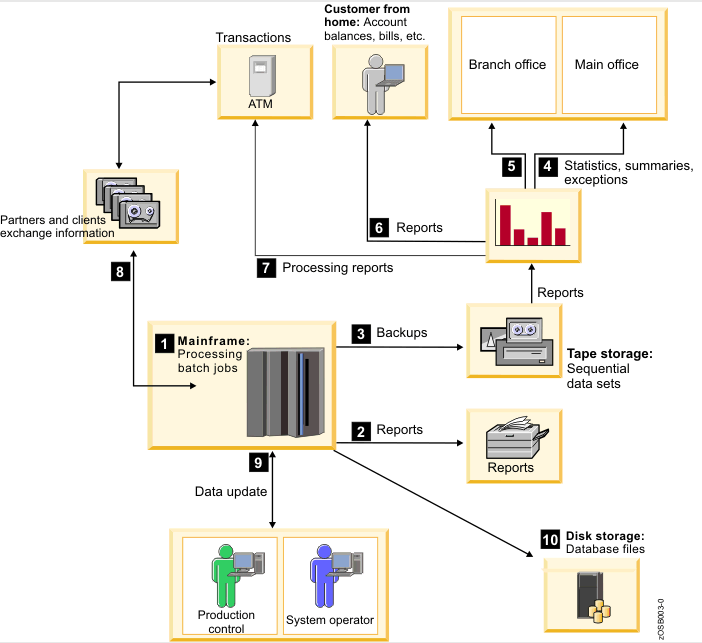
\includegraphics[width=400pt]{./graphics/BatchJobVB.png}
    \caption{Batch Job \autocite{IBMb}}
    \label{fig}
\end{figure}

\begin{itemize}
    \item[1] De batch job wordt opgestart door de mainframe
    \item[2] De job genereert statistieken van het bedrijf
    \item[3] Er wordt een backup gemaakt van de kritische bestanden en de database voor en na de job
    \item[4] De statistieken worden verstuurd naar een specifieke plaats zodat het geanalyseerd kan worden
    \item[5] Fouten of uitzonderingen in de statistieken worden in een andere locatie geplaatst
    \item[6] Informatie van klanten hun bankrekening wordt gemaakt en verstuurd.
    \item[7] Een verslag van de processing tijd wordt verstuurd naar de partners van de bank
    \item[8] De partner ontvangt het verslag
    \item[9] Het systeem monitort de uitkomst van de batch job
    \item[10] Jobs en transacties updaten de database zodat de progressie wordt opgeslagen
\end{itemize}
\\

Batch jobs zijn niet de enige vorm van jobs die uitgevoerd worden op een mainframe. Online transaction processing of OLTP is zeer belangrijk in een bank. In contrast met batch processing, heeft dit een eindgebruiker nodig die de job opstart. Het heeft ook geen vast moment waarop de job uitgevoerd wordt maar kan altijd doorheen de dag. Meestal duren deze transacties niet lang maar de systemen die verantwoordelijk zijn om deze jobs uit te voeren moeten veel verschillende gebruikers op hetzelfde moment moeten ondersteunen zonder enige vertraging. \autocite{IBMb} \\
Een grafische voorstelling van de verschillen tussen een batch job en een online transaction job vind u in figuur 4.2. \\ \\


\begin{figure}[pt!]
    \centering
    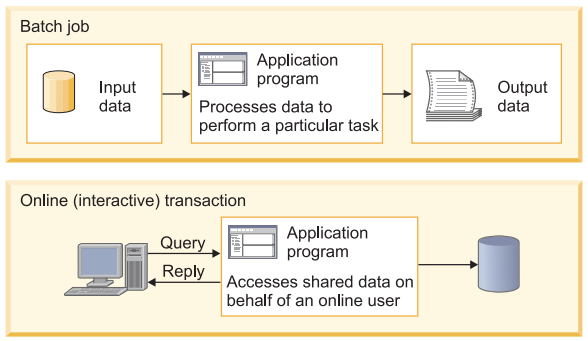
\includegraphics[width=400pt]{./graphics/BatchVSOnline.png}
    \caption{Grafisch verschil tussen batch en OLTP \autocite{IBMb}}
    \label{fig}
\end{figure}
%%=============================================================================
%% Opzetten Pydev in IDz
%%=============================================================================

\chapter{Opzetten Pydev}
\label{ch:opzetten-pydev}

In dit onderzoek zullen we een oudere versie vqn PyDev installeren namelijk PyDev 8.2.0 . Dit is een iets oudere versie maar het best compatibel met IDz, de andere versies kunnen problemen met zich meebrengen tijdens en na de installatie. Het programma waar het onderzoek in uitgevoerd zal worden is IBM Developer for z/OS (IDz) versie 16.0.2 met voorgeïnstalleerde programma's van DNB zelf. IDz is gebaseerd op Eclipse versie 4.23.0
Versie 8.2.0 bevat een debugger, een code formatter en code analyse. Het is belangrijk om te weten dat IDz door IBM beschikbaar wordt gesteld en ze dus support zullen bezorgen waar nodig moesten er problemen zijn met hun programma. Dit is niet het geval met PyDev omdat dit door een externe partij is ontwikkeld en dus niet ondersteund wordt door IBM. \\

\section{prerequisites}
\begin{itemize}
    \item Eclipse (versie 4.6) based programma nodig - IDz
    \item Java 11 of hoger
    \item Python 3.8 of hoger
\end{itemize}

\\
\\
\section{Installatie}
Om Pydev te gebruiken moeten we het eerst installeren via hun Github repository \url{https://github.com/fabioz/Pydev/releases} . Dit zal een .zip installeren die je moet uitpakken en ergens moet opslaan. Het uitpakken kan een enige tijd duren. \\

In IDz nqvigeer je naar help -> install New Software . Je zult een installatie wizard te zien krijgen en hierin klik je op add -> local en hier kies je dan de map waar Pydev in is uitgepakt. klik op add.

Je krijgt weer een scherm te zien met de opties die je kunt installeren. Het kan zijn dat het eerst leeg is en dit verander je door vanonder in de checkbox de Group items by categorieuit te vinken. Hierna krijg je 3 opties.

PyDev for Eclipse 8.2.0.202102211157
PyDev for Eclipse Developer Resources 8.2.0.202102211157
PyDev Mylyn Integration 0.6.0

De eerste is noodzakelijk en de tweede optioneel. De derde mag niet aangevinkt worden aangezien MyLyn niet is geïnstalleerd in IDz waardoor het opzetten van PyDev zal falen.

Klik op next, dit zal alles opzetten en kan even duren. Als dit gedaan is krijg je een overzicht van de installatie details en hier klik je op finish. In de balk rechtsonder kun je zien dat het bezig is met installeren.

Als het klaar is met installeren zal het een pop-up geven om IDz herop te starten. Als u nog open projecten heeft is het best om deze eerst op te slaan en dan zelf te herstarten. Anders klikt u nu op Restart Now

Om te zien of de installatie gelukt is navigeert u naar help -> about -> Installation details en zoekt u Pydev.
Hier zou u de geïnstalleerde software moeten zien


Als je een Python script opent zal het nogsteeds gebeuren in de interne text editor. Om dit te wijzigen moeten we de file associations bekijken. Deze zullen bepalen welke editor er gebruikt wordt bij een bepaalde extensie. Hier zullen we dus de Python editor van Pydev linken aan de .py extensie.

Ga naar Windos -> Preferences -> General -> Editors -> File Associations
Hier zie je een lijst met allemaal extensies en het programma waarmee ze geopend worden. IDz heeft niet standaard een python editor dus deze moeten we toevoegen door op add te klikken bij file types
Geef hier .py in en klik op ok

Je komt terug in de lijst van extensies en ziet hier normaal .py tussenstaan

Selecteer de py extensie en bij associated editors komen er 3 opties.
Deze opties worden gebruikt om bestanden met een .py extensie te openen


Als je een python script opent zal dit automatisch gebeuren in de python editor en heb je alle functies die Pydev te bieden heeft.
%In IDz navigeer je naar help -> Eclipse Marketplace. Hierin vind je dus allemaal verschillende plug-ins die je kunt gebruiken in IDz. In de zoekbalk zoek je 'Pydev', klik je op enter en dan install. Bij confirm selected features krijg je 2 opties en deze moeten allebei aangeklikt zijn. Hierna klik je op confirm




% Voeg hier je eigen hoofdstukken toe die de ``corpus'' van je bachelorproef
% vormen. De structuur en titels hangen af van je eigen onderzoek. Je kan bv.
% elke fase in je onderzoek in een apart hoofdstuk bespreken.

%\input{...}
%\input{...}
%...

%%=============================================================================
%% Conclusie
%%=============================================================================

\chapter{Conclusie}%
\label{ch:conclusie}

% TODO: Trek een duidelijke conclusie, in de vorm van een antwoord op de
% onderzoeksvra(a)g(en). Wat was jouw bijdrage aan het onderzoeksdomein en
% hoe biedt dit meerwaarde aan het vakgebied/doelgroep? 
% Reflecteer kritisch over het resultaat. In Engelse teksten wordt deze sectie
% ``Discussion'' genoemd. Had je deze uitkomst verwacht? Zijn er zaken die nog
% niet duidelijk zijn?
% Heeft het onderzoek geleid tot nieuwe vragen die uitnodigen tot verder 
%onderzoek?

Deze proof of concept biedt een meerwaarde aan de modernisatie van het mainframe systeem die sterk bezig is. Deze systemen zijn nog heel belangrijk, maar werken met te oude technieken waardoor er niet veel mensen zijn die ze kunnen onderhouden. Het toevoegen van modernere manieren van werken is niet voldoende, ze moeten ook efficiënt zijn om mee te kunnen werken, wat niet het geval is in de huidige versie van IDz. Dit kan opgelost worden door middel van de Pydev plug-in. \\

Het opstellen van deze plug-in is niet zeer complex, maar er zijn instellingen die niet voor de hand liggend zijn en voor problemen kunnen zorgen. Aangezien IDz ook veel verschillende functionaliteiten heeft, is het moeilijk om te weten waar er gezocht moet worden bij het opstellen van deze plug-in. \\

Het is zeer eenvoudig om applicaties te schrijven en direct te testen in hetzelfde programma. Door de Pydev plug-in is het schrijven zeer efficiënt. De terminal in Idz om Python-applicaties in uit te voeren daarentegen brengt wat problemen met zich mee die niet voorkomen in een externe ssh-connectie.
Tijdens het testen kwamen er problemen op bij iets complexere zaken, bijvoorbeeld het uitvoeren van de API of zelfs het opzetten van de Python virtuele omgeving. \\

Het hoofddoel van dit onderzoek was om een Python-interpreter op te zetten in IDz door middel van de Pydev plug-in wat goed gelukt is. Dit maakt het mogelijk om Python-applicaties direct te schrijven op de mainframe zonder een andere IDE te moeten gebruiken. Voor het opstellen werd er niet verwacht dat dit veel problemen met zich zou meebrengen behalve voor een paar instellingen. \\
Dit maakt het testen deels eenvoudiger, maar het wordt best gedaan in een externe ssh connectie om problemen te vermijden. Het is nog niet helemaal duidelijk wat de oorzaken zijn van de problemen in de terminal in IDz. \\

Dit onderzoek heeft duidelijk gemaakt dat Python compatibel is met de mainframe en nu is er ook een mogelijkheid om applicaties in deze programmeertaal direct te schrijven op de mainframe. Tools zoals ZOAU en de Python AI toolkit for z/OS maken de mogelijkheden enorm groot waardoor er zeer complexe applicaties geschreven kunnen worden. Door de afname van skills in COBOL en PL/1, is het interessant om te onderzoeken of Python en Java de oudere programmeertalen voor batch- en online-jobs volledig kunnen vervangen en of dit invloed zou hebben op de snelheid waarmee deze jobs worden uitgevoerd.



%---------- Bijlagen -----------------------------------------------------------

\appendix

\chapter{Onderzoeksvoorstel}

Het onderwerp van deze bachelorproef is gebaseerd op een onderzoeksvoorstel dat vooraf werd beoordeeld door de promotor. Dat voorstel is opgenomen in deze bijlage.

%% TODO: 
%\section*{Samenvatting}

% Kopieer en plak hier de samenvatting (abstract) van je onderzoeksvoorstel.

% Verwijzing naar het bestand met de inhoud van het onderzoeksvoorstel
%---------- Inleiding ---------------------------------------------------------
\newpage
\section{Introductie}%
\label{sec:introductie}
In de huidige technologische wereld is het moeilijk bij te houden welke mogelijkheden er zijn om bepaalde projecten uit te voeren. Zo heb je altijd nieuwe technieken die net iets efficiënter of krachtiger zijn dan een ander. Door deze voortgaande evolutie zullen individuen niet direct op de hoogte zijn van recente ontwikkelingen, maar vergeten ze ook de oudere toepassingen van een bepaalde techniek. Dit is vooral merkbaar bij IBM hun z Systems of mainframes die zo belangrijk, maar zo snel vergeten worden in de IT wereld. Hoewel het een zeer hoogwaardige technologie is, zijn de technieken nog steeds zeer oud. Hier wordt wel op ingezet door modernere talen zoals Java en Python compatibel te maken met dit systeem. Een veel gebruikte tool, aangeboden door IBM, is IBM Developer for z/OS. Dit is een Eclipse based programma geschreven in Java en kan een connectie maken met de mainframe en zijn opgeslagen bestanden. Dit maakt het eenvoudiger voor gebruikers om verschillende bestanden te openen maar heeft geen Python interpreter waardoor het voor developers niet zo efficiënt is om Python programma's aan te passen.


\subsection{Probleemstelling}
Het bedrijf waar het onderzoek in wordt uitgevoerd is Den Norske Bank (DNB) met een hoofdvestiging in Oslo, Noorwegen. Hun developers zoals Stian Botnevik zitten vast met het beschreven probleem en zoeken een efficiëntere manier om Python scripts te schrijven en testen. Momenteel passen ze Python scripts aan in een text editor van IBM Developer for z/OS (IDz) en testen ze de code in een ssh connectie. \\
Python scripts worden opgeslagen en uitgevoerd in de Unix System Services (USS) omgeving. Dit is een Unix omgeving op de mainframe. In IDz kunnen developers alle bestanden openen in de USS omgeving wat duidelijker is dan code aanpassen in een terminal via bijvoorbeeld de vim tool.  


%---------- Stand van zaken ---------------------------------------------------

\section{State-of-the-art}%
\label{sec:state-of-the-art}

\subsection{Een andere manier van werken}
Veel bedrijven die werken met een mainframe hebben het probleem dat ze onvoldoende mensen vinden met de nodige kennis over deze technologie. De introductie van Unix systemen op de mainframe in het jaar 2000 \autocite{Mertic2020} had dit probleem wat verminderd maar zeker niet weggewerkt. De oorzaak van deze situatie is door de oude technieken die het systeem gebruikt. COBOL en PL/1 zijn niet de meest aantrekkelijke programmeertalen om te leren en mensen kiezen liever Bash als scripttaal in plaats van REXX. Hoewel IBM veel inzet op documentatie en online leerplatformen zoals IBM Z Xplore, blijft het tekort van ervaren mensen nog steeds te laag. \\

De mainframe wereld zal zich dus moeten aanpassen aan de vaardigheden van de mensen door over te schakelen naar bekendere manieren van werken. 
Python bijvoorbeeld is een programmeertaal die steeds meer populariteit krijgt sinds zijn creatie in de vroege jaren 90 \autocite{Johnson2023}. Dit is niet enkel bij reeds ervaren programmeurs, maar mensen die net beginnen programmeren kiezen hier steeds vaker voor. Dit is vooral door zijn begin vriendelijkheid, verschillende doeleinden en een actieve community. \autocite{Johnson2023} \\

IBM heeft dit opgemerkt en een Python compiler en interpreter ontwikkeld voor z/OS genaamd IBM Open Enterprise SDK for Python. Hierdoor kun je met Python interactie hebben met z/OS om bijvoorbeeld applicaties te ontwikkelen of de resources van het systeem te gaan beheren. Door de Unix omgeving heeft de programmeur ook geen speciale z/OS kennis nodig. \autocite{Klaey2023} \\

\subsection{Bedrijven in het werkveld}
Een bank is een goed voorbeeld van een bedrijf die gebruik maakt van IBM hun mainframes. Dit valt te concluderen door het feit dat maar liefst 92 van de top 100 banken wereldwijd een mainframe gebruikt. Dit is ook logisch aangezien er gemiddeld 12.6 miljard financiële transacties per dag uitgevoerd worden. \autocite{Wagle2017} \\

Door dit aantal is de nood voor een mainframe toch niet te onderdrukken maar het is niet enkel het aantal transacties dat deze machine kan uitvoeren, het is ook de snelheid, schaalbaarheid en beveiliging van deze systemen dat een grote rol speelt. Het zijn ook niet enkel banken die van deze technologie gebruik maken, maar ook  verzekeringsmaatschappijen bijvoorbeeld. De top 10 van deze soort bedrijven maken allemaal gebruik van een IBM mainframe. \autocite{Tozzi2022}

\subsection{De Skill gap}
Het is nog steeds moeilijk om nieuw talent aan te trekken in de mainframe wereld. Een onderzoek van \textcite{Deloitte2020} toont aan dat 79\% van de projectleiders moeilijkheden heeft met het zoeken naar mensen met de juiste skillset. Hetzelfde onderzoek toont ook aan dat er in de teams zelf een groot verschil is van kennis en vaardigheden. Hoewel dit systeem gebruikt wordt door 71\% van de fortune 500 companies \autocite{Tozzi2022} , is de Skill gap nog steeds te groot waardoor veel bedrijven vrezen voor een groot tekort aan werknemers om deze z Systems te onderhouden. \\

Volgens Petra \textcite{Goude2023} zijn er verschillende manieren om dit probleem aan te pakken. Zo kunnen bedrijven lessen geven over mainframes en hoe ze dit gebruiken. Ze vertelt ook dat de vaardigheden die nodig zijn beter gecomplimenteerd moeten worden en kunnen leiden naar een belonende en lange termijn carrière. \\ 

Hoewel dit zou helpen, vind ze dit niet de kern van het probleem. Het zijn de oude technieken die mensen niet aantrekt. Ze stelt voor om meer te investeren in hedendaagse technologie en dit te installeren op de mainframe. Dit kan gaan over dezelfde test -en deployment technieken, maar ook over hedendaagse programmeertalen zoals Java of Python. Dit zou kunnen door middel van APIs en zou een nieuwe, jongere werkkracht aantrekken. \autocite{Goude2023}


\subsection{Toch nog een kleurrijke toekomst}
Ondanks de grote nood aan mensen met de juiste vaardigheden, ziet de toekomst er toch nog goed uit. Zo wordt er meer gemoderniseerd met bijvoorbeeld modernere programmeertalen. Er wordt ook voorspeld dat we een introductie van DevOps en self-service benaderingen gaan zien. \autocite{Pennaz2023} \\

Momenteel zijn Python en Java beschikbaar als programmeertaal op de mainframe naast PL/1 en COBOL.
Sinds deze introductie zijn al bijna 2/3de van gebruikers op de mainframe Java aan het toepassen op een bepaalde manier. \autocite{Watts2018}

% Voor literatuurverwijzingen zijn er twee belangrijke commando's:
% \autocite{KEY} => (Auteur, jaartal) Gebruik dit als de naam van de auteur
%   geen onderdeel is van de zin.
% \textcite{KEY} => Auteur (jaartal)  Gebruik dit als de auteursnaam wel een
%   functie heeft in de zin (bv. ``Uit onderzoek door Doll & Hill (1954) bleek
%   ...'')


%---------- Methodologie ------------------------------------------------------

\section{Methodologie}%
\label{sec:methodologie}
Deze paper zal als resultaat een volledig stappenplan geven om Pydev op te stellen in IDz en verdere configuratie om de scripts uit te voeren in IDz.

\subsection{Fase 1: Literatuurstudie}
\begin{itemize}
    \item \textbf{Doel:}
    Relevante informatie verzamelen van IDz, Pydev en de Unix System Services omgeving.
    \item \textbf{Aanpak:}
    \item[-] Opzoeken betrouwbare bronnen
    \item[-] Gelijke projecten onderzoeken
    \item[-] Overzicht van nodige software
    \item \textbf{Tijd:} 5 weken
    \item \textbf{Opbrengst:}
    Een volledig onderzoek naar vakliteratuur en nodige software die nodig is. Ook een volledige schets naar de omgeving waarin er wordt gewerkt.
\end{itemize}


\subsection{Fase 2: Opstellen Pydev}
\begin{itemize}
    \item \textbf{Doel:}
    Opzetten van de Pydev plug-in in IDz
    \item \textbf{Aanpak:}
    \item[-] De opgezochte literatuur bestuderen
    \item[-] Pydev opstellen met de juiste vereisten
    \item[-] Testen
    \item \textbf{Tijd:} 3 weken
    \item \textbf{Opbrengst:}
    Pydev voor functies zoals code completion, syntax check, code analysis, ... \\ 
    Bij het openen van een Python programma zal dit ook gebeuren via een Python editor
\end{itemize}


\subsection{Fase 3: Python interpreter opzetten}
\begin{itemize}
    \item \textbf{Doel:}
    Python Interpreter opstellen om Python programma's uit te voeren in IDz.
    \item \textbf{Aanpak:}
    \item[-] De opgezochte literatuur bestuderen met expert
    \item[-] Opzetten van de juiste interpreter
    \item[-] Testen
    
    \item \textbf{Tijd:} 2 weken
    \item \textbf{Opbrengst:}
    Python programma's kunnen uitvoeren in IDz.
\end{itemize}


\subsection{Fase 4: Verdere configuratie om de output van de mainframe in de IDz console te krijgen}
\begin{itemize}
    \item \textbf{Doel:}
    Onderzoeken welke functies er beschikbaar zijn in Pydev
    \item \textbf{Aanpak:}
    \item[-] Pydev documentatie bekijken
    \item[-] Zelf onderzoeken in IDz
    
    \item \textbf{Tijd:} 2 weken
    \item \textbf{Opbrengst:}
    Een overzicht van alle functies die beschikbaar zijn. 
\end{itemize}

\subsection{Fase 5: Evaluatie voorbereiding}
\begin{itemize}
    \item \textbf{Doel:}
    Eind evaluatie voorbereiden
    \item \textbf{Aanpak:}
    \item[-] Resultaat bespreken, vergelijken en concluderen
    \item[-] Op orde stellen van nodige documenten
    \item \textbf{Tijd:} 2 weken
    \item \textbf{Opbrengst:}
    Een eind evaluatie waarin de opdracht besproken wordt
\end{itemize}


%---------- Verwachte resultaten ----------------------------------------------
\section{Verwacht resultaat, conclusie}%
\label{sec:verwachte_resultaten}
Een volledig stappenplan voor de opstelling van Pydev en een Python interpreter die compatibel is met IDz. Ook zal de configuratie getoond worden om de output van Python programma's te zien in IDz. Hierbij zal er bij elke stap uitleg gegeven worden over waarom het op die bepaalde manier gedaan wordt. Ook zal er besproken worden wat er mogelijks mis zou kunnen gaan. Screenshots zullen gebruikt worden voor duidelijk te maken wat er gebeurd. \\ 

Door de Pydev plug-in zal de interpreter eenvoudig opgesteld kunnen worden. Hier worden wel wat problemen verwacht omdat Pydev voor standaard Eclipse is ontwikkeld en IDz is hier een afstamming van waardoor er bepaalde onderdelen anders kunnen zijn. 


 

%%---------- Andere bijlagen --------------------------------------------------
% TODO: Voeg hier eventuele andere bijlagen toe. Bv. als je deze BP voor de
% tweede keer indient, een overzicht van de verbeteringen t.o.v. het origineel.
%\input{...}

%%---------- Backmatter, referentielijst ---------------------------------------

\backmatter{}

\setlength\bibitemsep{2pt} %% Add Some space between the bibliograpy entries
\printbibliography[heading=bibintoc]

\end{document}
